\documentclass{article}
\usepackage{graphicx}
\usepackage[margin=1.0in]{geometry}

\title{Vector DM Merging Soliton Test}
\author{Philip Mocz}

\begin{document}

\maketitle

\begin{figure}[ht]
\begin{tabular}{cccc}
$N$ & $\psi_1$ & $\psi_2$ & $\psi_3$ \\
$32$ & 
\includegraphics[width=0.24\textwidth]{s42r32s20psi1.png} &
\includegraphics[width=0.24\textwidth]{s42r32s20psi2.png} &
\includegraphics[width=0.24\textwidth]{s42r32s20psi3.png} \\
$64$ & 
\includegraphics[width=0.24\textwidth]{s42r64s20psi1.png} &
\includegraphics[width=0.24\textwidth]{s42r64s20psi2.png} &
\includegraphics[width=0.24\textwidth]{s42r64s20psi3.png} \\
$128$ & 
\includegraphics[width=0.24\textwidth]{s42r128s20psi1.png} &
\includegraphics[width=0.24\textwidth]{s42r128s20psi2.png} &
\includegraphics[width=0.24\textwidth]{s42r128s20psi3.png} \\
\end{tabular}
\caption{Plot of projected densities at the end of simulation ($t=2$).}
\end{figure}


\begin{figure}[ht]
\begin{tabular}{cccc}
$N$ & $\psi_1$ & $\psi_2$ & $\psi_3$ \\
$32$ & 
\includegraphics[width=0.24\textwidth]{s42r32s20psi1_phase.png} &
\includegraphics[width=0.24\textwidth]{s42r32s20psi2_phase.png} &
\includegraphics[width=0.24\textwidth]{s42r32s20psi3_phase.png} \\
$64$ & 
\includegraphics[width=0.24\textwidth]{s42r64s20psi1_phase.png} &
\includegraphics[width=0.24\textwidth]{s42r64s20psi2_phase.png} &
\includegraphics[width=0.24\textwidth]{s42r64s20psi3_phase.png} \\
$128$ & 
\includegraphics[width=0.24\textwidth]{s42r128s20psi1_phase.png} &
\includegraphics[width=0.24\textwidth]{s42r128s20psi2_phase.png} &
\includegraphics[width=0.24\textwidth]{s42r128s20psi3_phase.png} \\
\end{tabular}
\caption{Plot of slice of phase (plotted as $\cos\left({\rm arg}\left(\psi\right)\right)$) at the end of simulation ($t=2$).}
\end{figure}


\begin{figure}[ht]
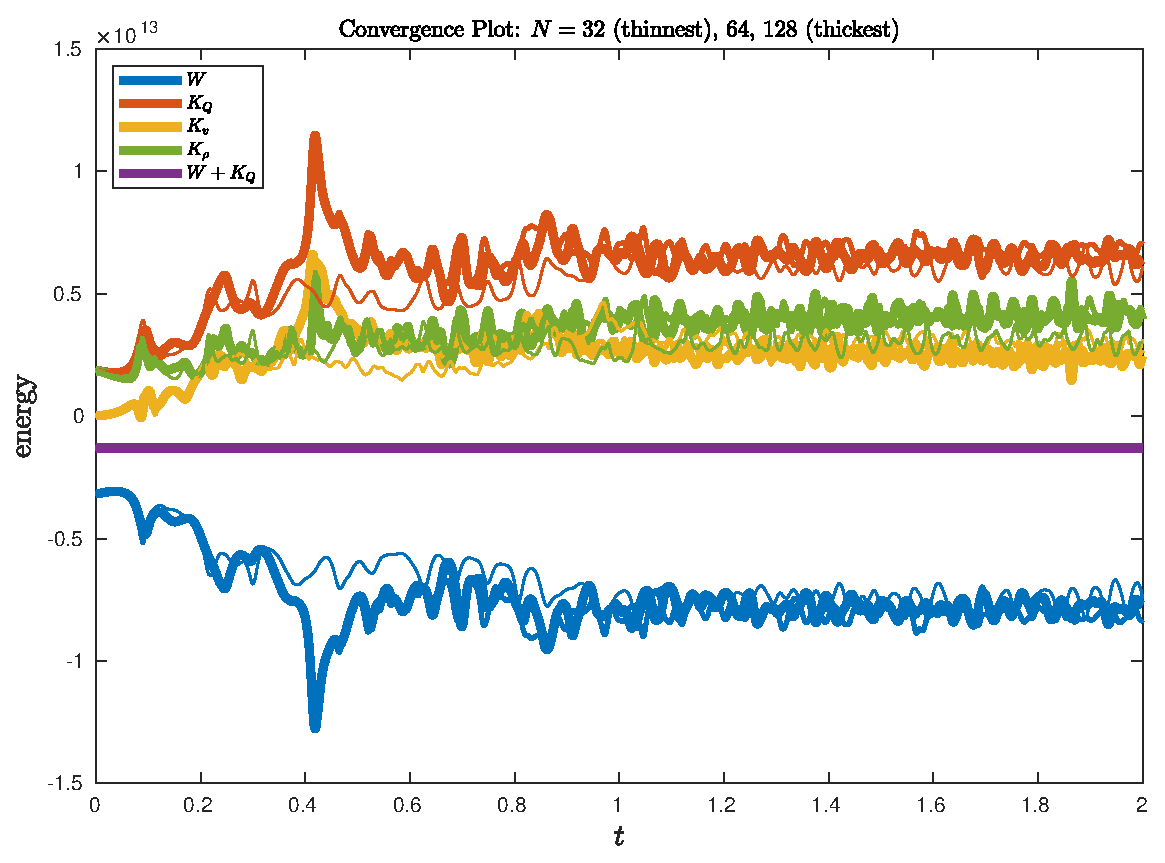
\includegraphics[width=0.7\textwidth]{energies2.eps} 
\caption{Plot of energies.}
\end{figure}


\end{document}
